

\tikzset{every picture/.style={line width=0.75pt}} %set default line width to 0.75pt        

\begin{tikzpicture}[x=0.75pt,y=0.75pt,yscale=-0.8,xscale=0.8]
%uncomment if require: \path (0,300); %set diagram left start at 0, and has height of 300

%Shape: Triangle [id:dp6057132058653998] 
\draw   (265.5,90) -- (400.5,228) -- (205,228) -- cycle ;
\draw  [fill={rgb, 255:red, 0; green, 0; blue, 0 }  ,fill opacity=1 ] (294,221) -- (306.5,227.5) -- (294,234) -- (300.25,227.5) -- cycle ;
\draw  [fill={rgb, 255:red, 0; green, 0; blue, 0 }  ,fill opacity=1 ] (225.47,162.57) -- (237.43,155.12) -- (236.66,169.19) -- (234.25,160.5) -- cycle ;
%Straight Lines [id:da5161540821426658] 
\draw    (205,228) -- (325.5,152) ;
\draw  [fill={rgb, 255:red, 0; green, 0; blue, 0 }  ,fill opacity=1 ] (281.46,172.5) -- (295.47,171.07) -- (288.59,183.36) -- (290.25,174.5) -- cycle ;
%Shape: Brace [id:dp2907792729734002] 
\draw   (268,92) .. controls (264.6,95.2) and (264.5,98.5) .. (267.7,101.89) -- (283.8,119.01) .. controls (288.37,123.87) and (288.95,127.9) .. (285.55,131.09) .. controls (288.95,127.9) and (292.93,128.73) .. (297.5,133.58)(295.45,131.39) -- (313.61,150.7) .. controls (316.8,154.1) and (320.1,154.2) .. (323.5,151) ;
%Shape: Brace [id:dp31460660756332137] 
\draw   (412.5,215) .. controls (415.87,211.77) and (415.95,208.47) .. (412.72,205.1) -- (359.47,149.39) .. controls (354.86,144.58) and (354.25,140.56) .. (357.62,137.33) .. controls (354.25,140.56) and (350.26,139.76) .. (345.65,134.94)(347.72,137.11) -- (292.39,79.23) .. controls (289.16,75.86) and (285.86,75.78) .. (282.49,79) ;
\draw  [fill={rgb, 255:red, 0; green, 0; blue, 0 }  ,fill opacity=1 ] (359.62,195.5) -- (356.06,181.86) -- (369.26,186.78) -- (360.25,186.5) -- cycle ;
%Shape: Brace [id:dp8011846743806035] 
\draw   (328.5,153) .. controls (325.11,156.21) and (325.01,159.51) .. (328.22,162.9) -- (350.54,186.54) .. controls (355.12,191.39) and (355.71,195.41) .. (352.32,198.61) .. controls (355.71,195.41) and (359.7,196.23) .. (364.27,201.08)(362.21,198.9) -- (386.6,224.72) .. controls (389.81,228.11) and (393.11,228.21) .. (396.5,225) ;
%Straight Lines [id:da6231155430584114] 
\draw    (457,86) -- (483.02,109.65) ;
\draw [shift={(484.5,111)}, rotate = 222.27] [color={rgb, 255:red, 0; green, 0; blue, 0 }  ][line width=0.75]    (10.93,-3.29) .. controls (6.95,-1.4) and (3.31,-0.3) .. (0,0) .. controls (3.31,0.3) and (6.95,1.4) .. (10.93,3.29)   ;
%Straight Lines [id:da6271046257844906] 
\draw    (456.5,109.5) -- (483.42,88.72) ;
\draw [shift={(485,87.5)}, rotate = 502.33] [color={rgb, 255:red, 0; green, 0; blue, 0 }  ][line width=0.75]    (10.93,-3.29) .. controls (6.95,-1.4) and (3.31,-0.3) .. (0,0) .. controls (3.31,0.3) and (6.95,1.4) .. (10.93,3.29)   ;
\draw  [fill={rgb, 255:red, 0; green, 0; blue, 0 }  ,fill opacity=1 ] (292.62,127.5) -- (289.06,113.86) -- (302.26,118.78) -- (293.25,118.5) -- cycle ;

% Text Node
\draw (185,228.4) node [anchor=north west][inner sep=0.75pt]    {$O$};
% Text Node
\draw (393,231.4) node [anchor=north west][inner sep=0.75pt]    {$A$};
% Text Node
\draw (250,74.4) node [anchor=north west][inner sep=0.75pt]    {$C$};
% Text Node
\draw (308,230.4) node [anchor=north west][inner sep=0.75pt]    {$\underline{a}$};
% Text Node
\draw (211,129.4) node [anchor=north west][inner sep=0.75pt]    {$\underline{c}$};
% Text Node
\draw (255,166.4) node [anchor=north west][inner sep=0.75pt]    {$\underline{b}$};
% Text Node
\draw (326,136.4) node [anchor=north west][inner sep=0.75pt]    {$B$};
% Text Node
\draw (269,129.4) node [anchor=north west][inner sep=0.75pt]    {$n$};
% Text Node
\draw (360,121.4) node [anchor=north west][inner sep=0.75pt]    {$m$};
% Text Node
\draw (295,192.4) node [anchor=north west][inner sep=0.75pt]    {$m-n$};
% Text Node
\draw (414,145.4) node [anchor=north west][inner sep=0.75pt]    {$\underline{c} =\dfrac{m\underline{b} -n\underline{a}}{m-n}$};
% Text Node
\draw (439,69.4) node [anchor=north west][inner sep=0.75pt]    {$m$};
% Text Node
\draw (486,69.4) node [anchor=north west][inner sep=0.75pt]    {$n$};
% Text Node
\draw (441,104.4) node [anchor=north west][inner sep=0.75pt]    {$\underline{a}$};
% Text Node
\draw (486,106.4) node [anchor=north west][inner sep=0.75pt]    {$\underline{b}$};


\end{tikzpicture}